\ifx\fulldocument\undefined
\documentclass[aspectratio=169]{beamer}
% \usetheme{sdr}
\graphicspath{{./tex/imgs/}}

\usepackage[utf8]{inputenc}

\title{Programmiamo Umanoidi!}
\subtitle{}
\author{Lorenzo Leonardini}
\institute{Scuola di Robotica}
\date{\today}

\begin{document}

\begin{frame}
	\titlepage
\end{frame}

\section{Che cos'è NAO}
\subsection{Caratteristiche}
\subsection{Movimento}
\subsection{Utilizzi}
\subsection{Software}
\section{Choregraphe}
\section{Primo programma}

\AtBeginSection[]
{
\begin{frame}{Indice}
\tableofcontents[currentsection]
\end{frame}
}
\fi

\section{NAO Actor Studio}

\begin{frame}
\frametitle{NAO Actor Studio}
\begin{columns}
	\column{0.5\textwidth}
		Obiettivi:
		\begin{itemize}
			\item<2-> Far recitare a NAO la scena di un film
		\end{itemize}
	\column{0.5\textwidth}
		\begin{figure}[ht]
		\begin{center}
		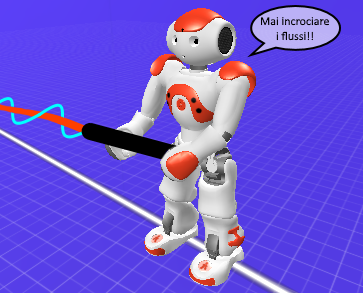
\includegraphics[width=.9\textwidth]{flussi}<2->
		\end{center}
		\end{figure}
\end{columns}
\end{frame}

\begin{frame}
\frametitle{NAO Actor Studio}
\begin{columns}
	\column{0.5\textwidth}
		Come:
		\begin{itemize}
			\item<2-> Scegliere la scena di un film
			\item<3-> Scaricare l'audio della scena da internet
			\item<4-> Registrare un animazione
			\item<5-> Eseguire l'animazione e riprodurre l'audio contemporaneamente
		\end{itemize}
	\column{0.5\textwidth}
		\begin{figure}[ht]
		\begin{center}
		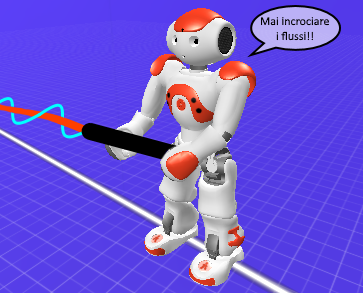
\includegraphics[width=.9\textwidth]{flussi}<1->
		\end{center}
		\end{figure}
\end{columns}
\end{frame}

\begin{frame}
\frametitle{Choregraphe}
\begin{figure}[ht]
\begin{center}
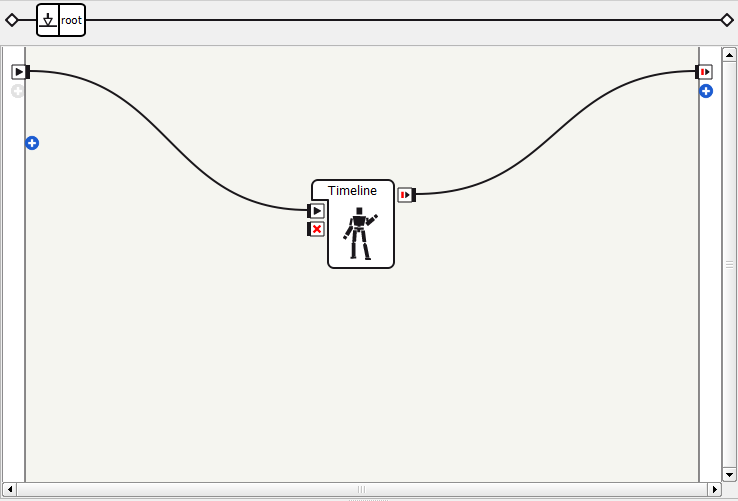
\includegraphics[width=.6\textwidth]{animation}
~\footnote{Il blocco Timeline}
\end{center}
\end{figure}
\end{frame}

\begin{frame}
\frametitle{Choregraphe}
\begin{figure}[ht]
\begin{center}
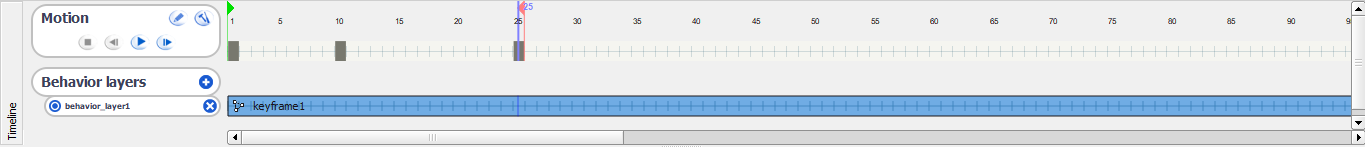
\includegraphics[width=\textwidth]{timeline}
~\footnote{Contenuto del blocco}
\end{center}
\end{figure}
\end{frame}

\ifx\fulldocument\undefined
\end{document}
\fi
